\documentclass[12pt]{article}
\usepackage{graphicx}
\usepackage{subcaption}
\usepackage[parfill]{parskip}    		% Activate to begin paragraphs with an empty line rather than an indent
\usepackage{graphicx}				% Use pdf, png, jpg, or eps§ with pdflatex; use eps in DVI mode
\graphicspath{ {images/} }
\usepackage[margin=1in]{geometry}
\usepackage{float}
\usepackage{amsmath}
\usepackage{amssymb}
\title{Propagation of Voltage in a Neuron: The Cable Equation}
\author{Darice Guittet, Elise Niedringhaus, Sarah Liddle}

\begin{document}
\maketitle
\section{Introduction}

Information within the brain is transmitted between neurons largely as a result of action potentionals, otherwise known as spikes, which are when the voltage in a neuron rapidly rises and falls. A.L Hodgkin and A.F. Huxley received a 1963 Nobel Prize for their work regarding this topic, specifically the discovery that individual parts of the axonal membrane behave similarly to a component in an electric circuit. With this new knowledge, it is now possible to derive equations that represent the voltage propagation in a neuron using formulas similar to those that describe current, resistance, and voltage in an electrical system. This pattern of voltage diffusion along the membrane of neurons is called neuronal cable theory, which is what we will be analyzing in this report.

\subsection{Understanding the Model}
The model we are using to understand the propagation of voltage in a neuron can be described by the following partial differential equation:
\begin{equation} \label{1}
\frac{\partial{v(x,t)}}{\partial{t}}=\frac{\partial^2{v(x,t)}}{\partial{x}^2}+f(v(x,t))+J_{ext}(x,t)
\end {equation}
The terms with partial derivatives are from the diffusion equation, mathematically describing the process when molecules move from areas of high concentration to places of low concentration. The $f(v(x,t))$ term accounts for ion channels in a neuron; these open and close in response to the cell's current voltage. The $J_{ext}(x,t)$ term accounts for the external voltage that is applied to the neuron. 
\subsubsection{Summary of the Derivation}
We will take the membrane to be an infitesimal segment $[x, x+dx]$ with separate intra- and extracellular voltages and resistances, denoted by either an $i$ or an $e$ in the subscript, respectively. The first step in deriving the model is using Ohm's law to relate current, voltage, and resistance. Note that since we will be examining the voltage in the membrane of a neuron, it is important to examine each of these values inside and outside of the cell; this results in two equations for current. 
\[v_i(x+dx)-v_i(x)=-I_i(x)R_idx\]
\[v_e(x+dx)-v_e(x)=-I_e(x)R_edx\]
If we take these relations, divide by $dx$,  take the limit as $dx\rightarrow 0$, and solve for current, we get the following equations:
\[I_i(x)=-\frac{\partial}{\partial{x}}(\frac{1}{R_i(x)}\frac{\partial{v_i}}{\partial{x}})\]
\[I_e(x)=-\frac{\partial}{\partial{x}}(\frac{1}{R_e(x)}\frac{\partial{v_e}}{\partial{x}})\]
Now, we want to use these two equations to solve for the current per unit length $J_m(x)$, where, for an infinitesimal segment, $J_m(x)dx=I_e(x+dx)-I_e(x)=I_i(x)-I_i(x+dx)$. We will divide by $dx$ and take the limit as $dx\rightarrow 0$. This gives the relationship:
\[J_m(x)=\frac{\partial{I_e}}{\partial{x}}=-\frac{\partial{I_i}}{\partial{x}}\]
The voltage across the cell membrane must be the difference between the intra- and extracellular voltages: $v=v_i-v_e$ and the sum of intra- and extracellular currents yields a total constant current that will be equal to the sum of the intra- and extracellular current. We will use Ohm's law to write this current in terms of resistance and voltage, rewriting voltages with the relation $v=v_i-v_e$, and plug all these into the sum of currents equation, which must be constant. We take the partial derivative with respect to x and get the following relationship between current per unit length $J_m(x)$ and voltage $v$.
\begin{equation} \label{2}
J_m(x)=\frac{\partial}{\partial{x}}\bigg(\frac{1}{R(x)}\frac{\partial{v}}{\partial{x}}\bigg)
\end {equation}
This describes the current passing through the membrane of a neuron and is also a form of the diffusion equation.\par
Now, we will consider time variables in this model because the model behaves like an RC circuit and possesses some nonlinear properties of ion channels that act similarly to resistors. When the current per unit length has a time variable, it is also the sum of capactive current, outward ionic current, and inward applied current. If we plug this relation into Equation (\ref{2}), we get the following:
\[C\frac{\partial{v(x,t)}}{\partial{t}}=-J_{ION}(v(x,t),t)+\frac{1}{R}\frac{\partial^2{v(x,t)}}{\partial{x}^2}+J_A(x,t)\]
The outward applied current term, $-J_{ION}(v(x,t),t)$ , can be represented by $f(v(x,t))$, a nonlinear function that controls how voltage leaves or enters the system. The term $J_A(x,t)$ is the inward applied current, and represents the voltage applied to the system externally. After rescaling to get rid of $R$ and $C$ and renaming variables as $x$ and $t$, the final model becomes:
\[\frac{\partial{v(x,t)}}{\partial{t}}=\frac{\partial^2{v(x,t)}}{\partial{x}^2}+f(v(x,t))+J_{ext}(x,t)\]

\subsection{Purpose}
In this project, we first look at a passive membrane where there is no voltage gradient and ions leak out of the cell. We solve the stationary solution and then solve the partial differential equation in order to analyze the impulse propagation reaction to various initial voltage inputs. In the second section, we analyze a nonlinear model that takes into account the two-state nature of ion channels, one inactive and one active. We use these to examine the traveling wave solutions of this model and explore the effects of various conditions and inputs on the voltage propagation within a neuron.
\section{Passive Membrane}
We consider a passive membrane current with a linear ionic current that obeys Ohm's Law, with the resistance rescaled to unity: $f(v(x,t)) = -v(x,t)$. In addition, we add an external impulse at $x=0$ and $t=0$, formulated as the dirac delta function $\delta(t) \delta(x)$, to examine how the voltage responds. Since axons are much longer than they are wide, $x$ will range from $-\infty$ to $\infty$. We are also looking for bounded solutions since this is a physical system, therefore we look for solutions such that $\int_{-\infty}^{\infty}|v(x,t)|dx = M < \infty$. The inhomogeneous PDE corresponding to such a system is given by
\begin{equation} \label{pm}
\frac{\partial{v(x,t)}}{\partial{t}}=\frac{\partial^2{v(x,t)}}{\partial{x}^2}-v(x,t)+\delta(t)\delta(x)
\end {equation}

\subsection{Stationary Solutions}
To start, we find the stationary solutions, $v(x,t) = V_0(x)$, satisfying $\frac{\partial{v(x,t)}}{\partial{t}} = 0$ by solving the homogeneous ODE:
\begin{equation} \label{pm_odeH}
\frac{d^2{V_0(x)}}{d{x^2}} - V_0(x) = 0
\end{equation}
The general solution is $V_0(x) = c_1e^{-x} + c_2e^{x}$. However, in order for $V_0$ to be bounded on $(-\infty, \infty)$, $V_0$ = 0:

\subsection{Impulse Response}
We add a stationary input current localized at $x=0$ and find solutions $V_F(x)$ to the resulting inhomogeneous ODE with boundary conditions $\lim_{x\to\infty} V_F(x) = 0$.
\begin{equation} \label{pm_odeN}
\frac{d^2{V_F(x)}}{d{x^2}} - V_F(x) = -\delta(x)
\end{equation}
We compute the Fourier transforms of the ODE to find an algebraic equation for the Fourier transform of the solution $\mathcal{FT}\left\{V_F(x)\right\} = \overline{V_F}(\omega)$, where $\omega$ is the spatial frequency with units $\frac{1}{x}$. Using the fact that $\mathcal{FT}\left\{d_{xx}V_F(x)\right\} = -\omega^2\overline{V_F}(\omega)$ and $ \mathcal{FT}\left\{\delta(x)\right\} = 1$, we get an equation which we can rearrange into:
$$  \overline{V_F}(\omega) = \frac{1}{\omega^2+1} $$
From a Fourier transform table \cite{fourier}, we find our solution to be:
$$ V_F(x) = \mathcal{FT}^{-1}\left\{\overline{V_F(\omega)}\right\} =  \frac{1}{2}e^{-|x|} $$

\subsection{Generalizing Solutions}
If we make the change of variable $x = x-x_0$ to Part 2.2, we arrive at the inhomogeneous ODE whose solution is defined to be Green's function for this particular problem. Let $\mathcal{L}\left\{G\right\}$ be the linear operator that is the left-hand side of the equation and $G(x-x_0)$ be Green's function, satisfying the same boundary conditions as above.
\begin{equation} \label{pm_greens}
\mathcal{L}\left\{G\right\} = -\frac{d^2{G(x-x_0)}}{d{x^2}} + G(x-x_0) = \delta(x-x_0)
\end{equation}
$$ G(x-x_0) = \frac{1}{2}e^{-| x-x_0 |} $$
For any external input $f(x)$ and the associated inhomogeneous equation $\mathcal{L}\left\{y\right\} = f(x)$, the solution $y(x)$ can be found as
$$ y(x) = \int_{a}^{b}G(x-x_0)f(x_0)dx_0 $$
This fundamental property of Green's function is due to the \textit{sifting property} of the dirac delta function. 
$$\mathcal{L}\left\{y\right\} = L\int_a^bG(x-x_0)f(x_0)dx_0 = \int_a^b\mathcal{L}\left\{G(x-x_0)\right\}f(x_0)dx_0 = \int_a^b\delta(x-x_0)f(x_0)dx_0 $$
The formula for a stationary solution given an arbitrary stationary input uses Green's function as below.
$$V_A(x) = \int_{-\infty}^{\infty}\frac{1}{2}e^{-|x-x_0|}J_{ext}(x_0)dx_0 $$

\subsection{Green's Function for Time-Dependent Equation}
Returning to the full time-dependent equation (\ref{pm}), we again use Fourier transforms to find the solution, $G_{\infty}(x,t)$, Green's function on the infinite cable. This time, the Fourier transform of the PDE results in an inhomogeneous ODE for $\overline{G_{\infty}}(\omega,t)$.
\begin{equation}\label{pm_timeFT}
\frac{d}{dt}\overline{G_{\infty}}(\omega,t) + (\omega^2+1)\overline{G_{\infty}}(\omega,t) = \delta(t) 
\end{equation} 
When $t>0$, $\delta(t) = 0$ so the equation is reduced to a homogeneous ODE. Separation of variables and integration of both sides leads to the homogeneous solution, scaled by a function that is only dependent on $\omega$.
$$ \int\frac{1}{\overline{G_{\infty}}(\omega,t)}d\overline{G_{\infty}}(\omega,t) = -\int(\omega^2 + 1)dt $$

$$ \ln|(\overline{G_{\infty}}(\omega,t)| = -(\omega^2+1)t + c(\omega) $$
 
$$\overline{G_{\infty}}(\omega,t) = c(\omega)e^{-t(\omega^2+1)} $$
To find the value of $c(\omega)$, we examine the solution around $t=0$. Due to $\delta(t)$, there is a discontinuity such that $\lim_{\epsilon \to 0}\overline{G_{\infty}}(\omega,\epsilon^-) = 0$ due to the fact that our system starts at $t=0$, while $\lim_{\epsilon \to 0}\overline{G_{\infty}}(\omega,\epsilon^+) = c(\omega)$. We integrate equation (\ref{pm_timeFT}) at a small section around the discontinuity, from $t=(-\epsilon, \epsilon)$. 
$$\int_{-\epsilon}^{\epsilon}\frac{d}{dt}\overline{G_{\infty}}(\omega,t)dt + \int_{-\epsilon}^{\epsilon}(\omega^2+1)\overline{G_{\infty}}(\omega,t)dt = \int_{-\epsilon}^{\epsilon}\delta(t)dt $$

$$  \overline{G_{\infty}}(\omega,\epsilon) + \int_{-\epsilon}^{\epsilon}(\omega^2+1)\overline{G_{\infty}}(\omega,t)dt = 1$$
Taking the limit as $\epsilon \to 0$, we find the integral goes to zero and we are left with the constraint.
$$ \lim_{\epsilon\to 0} \overline{G_{\infty}}(\omega,\epsilon)  = \lim_{t\to 0^+}c(\omega)e^{-t(\omega^2+1)}  = 1 $$
Therefore, $c(\omega) = 1$ and compute the inverse Fourier transform for solution for $t>0$ by completing the square for the exponents and recognizing the result as a Gaussian integral.
$$\mathcal{FT}^{-1}\left\{\overline{G_{\infty}}(\omega,t)\right\} = \frac{1}{2\pi}\int_{-\infty}^{\infty}e^{-t(\omega^2+1)}e^{i \omega x)} d\omega = \frac{1}{2\pi}\int_{-\infty}^{\infty}e^{i \omega x-t(\omega^2+1)}d\omega $$

$$ G_{\infty}(x,t) = \frac{\mathcal{H}(x,t)}{2\pi}e^{-t-\frac{x^2}{4t}}\int_{-\infty}^{\infty}e^{-t(\omega - \frac{ix}{2t} )^2 }d\omega = \frac{\mathcal{H}(x,t)}{\sqrt{4\pi t}}e^{-t-\frac{x^2}{4t}} $$

\subsubsection{Plots of Green's Function}
We plot Green's function at $t=0$, $t=1$, $t=10$ and $t=100$.

\begin{figure}[H]
    \centering
    \begin{subfigure}[h]{0.4\textwidth}
        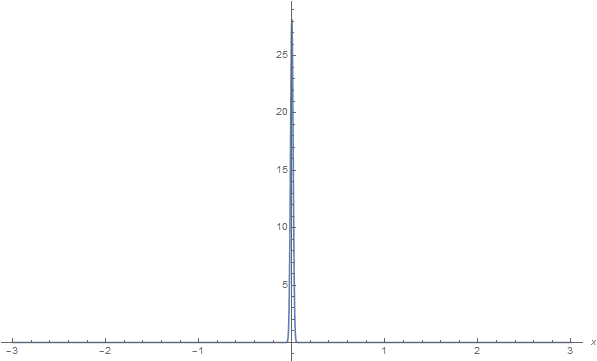
\includegraphics[width=\textwidth]{Part1Plots/t0}
        \caption{$t=0$}
        \label{fig:t0}
    \end{subfigure}
    \begin{subfigure}[h]{0.4\textwidth}
        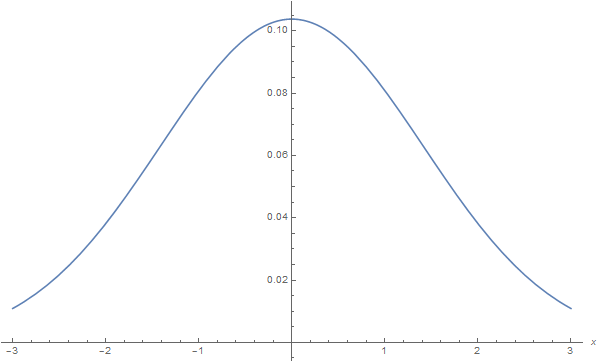
\includegraphics[width=\textwidth]{Part1Plots/t1}
        \caption{$t=1$}
        \label{fig:t1}
    \end{subfigure}
    \begin{subfigure}[h]{0.4\textwidth}
        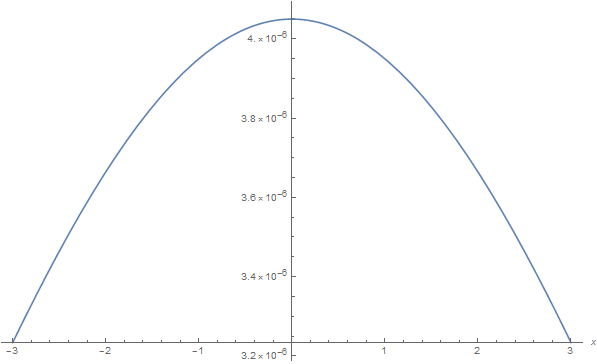
\includegraphics[width=\textwidth]{Part1Plots/t10}
        \caption{$t=10$}
        \label{fig:t10}
    \end{subfigure}
    \begin{subfigure}[h]{0.4\textwidth}
        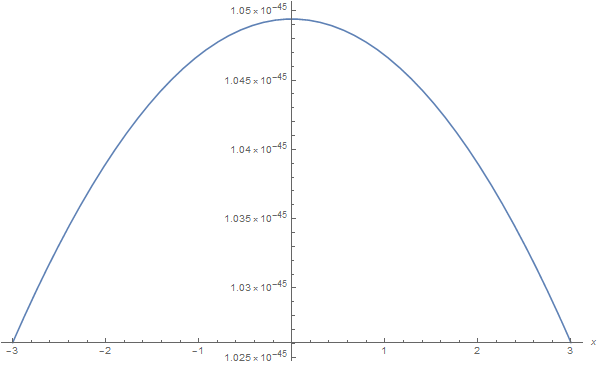
\includegraphics[width=\textwidth]{Part1Plots/t100}
        \caption{$t=100$}
        \label{fig:t100}
    \end{subfigure}
    \caption{Plots of Green's Function at Various Times}\label{fig:timeplots}
\end{figure}

We also plot Green's function at $x=0$, where voltage is monotone decreasing, and $x=2$, where voltage is nonmonotonic, for $t>0$.

\begin{figure}[H]
    \centering
    \begin{subfigure}[h]{0.4\textwidth}
        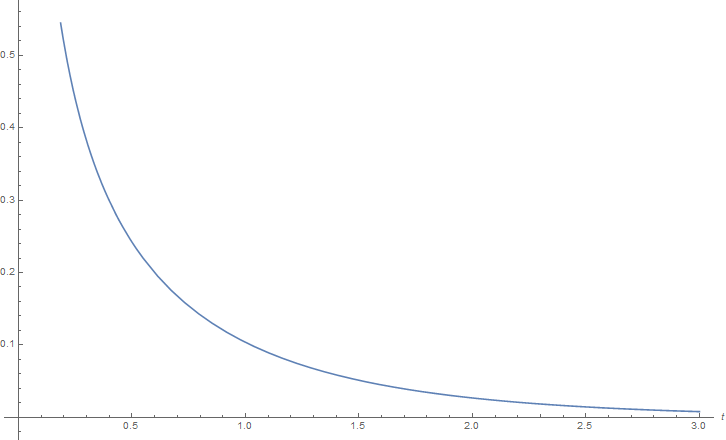
\includegraphics[width=\textwidth]{Part1Plots/x0}
        \caption{$x=0$}
        \label{fig:x0}
    \end{subfigure}
    \begin{subfigure}[h]{0.4\textwidth}
        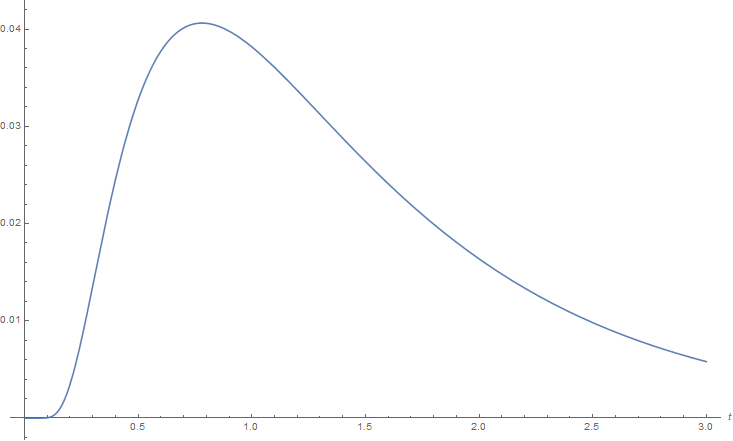
\includegraphics[width=\textwidth]{Part1Plots/x2}
        \caption{$x=2$}
        \label{fig:x2}
    \end{subfigure}

    \caption{Plots of Green's Function at Various Locations}\label{fig:spaceplots}
\end{figure}

The total voltage was computed to be $\int_{-\infty}^{\infty}G_{\infty}(x,t)dx = e^{-t}, t>0$ and it is monotone decreasing.

\begin{figure}[H]
	\centering
	\begin{subfigure}[h]{0.8\textwidth}
        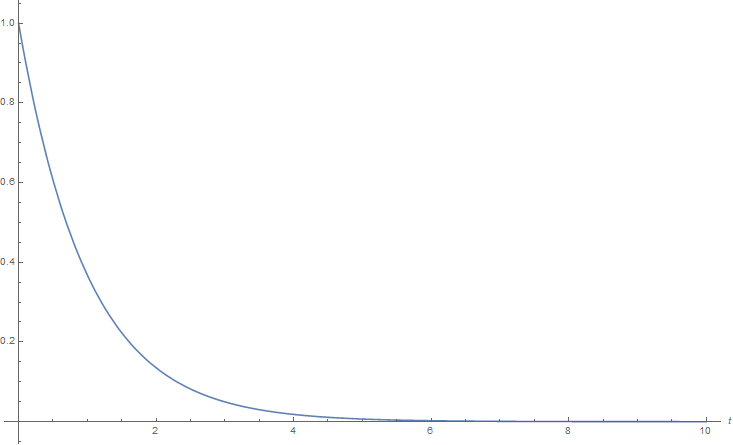
\includegraphics[width=\textwidth]{Part1Plots/g}
    \end{subfigure}
    \caption{Total Voltage} \label{fig:totalvoltage}
\end{figure}
   	
   	
\subsection{Generalizing Solutions}
Using Green's function found above, the formula for a generalized solution given arbitrary spatiotemporal input $J_{ext}(x,t)$ is

$$ \int_{-\infty}^{\infty}\int_{-\infty}^{\infty}G_{\infty}(x-x_0,t-t_0)J_{ext}(x_0,t_0)dx_0dt_0 $$

\pagebreak

\subsubsection{Example Function 1}
For $J_{1}(x,t) = [\delta(x-1)+\delta(x+1)]\delta(t)$, with a starting momentary impulse at $x=1$ and $x=-1$ , the solution is found and plotted below.

$$ v_1(x,t) = \frac{\mathcal{H}(t)}{2\sqrt{\pi t}}(1+e^{\frac{x}{t}})e^{-t-\frac{(1+x)^2}{4t}} $$

\begin{figure}[H]
	\centering
	\begin{subfigure}[h]{0.8\textwidth}
        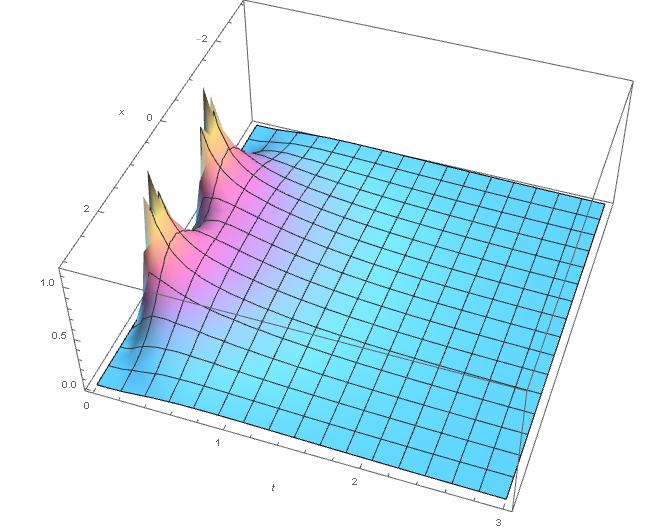
\includegraphics[width=\textwidth]{Part1Plots/plot1}
    \end{subfigure}
    \caption{Plot of $v_1(x,t)$ with $J_{1}(x,t)=[\delta(x-1)+\delta(x+1)]\delta(t)$} \label{fig:jext1}
\end{figure}

\pagebreak
\subsubsection{Example Function 2}
For $J_{2}(x,t) = 1$, the solution and plot is:
$$ v_2(x,t) = 1 $$

\begin{figure}[H]
	\centering
	\begin{subfigure}[h]{0.8\textwidth}
        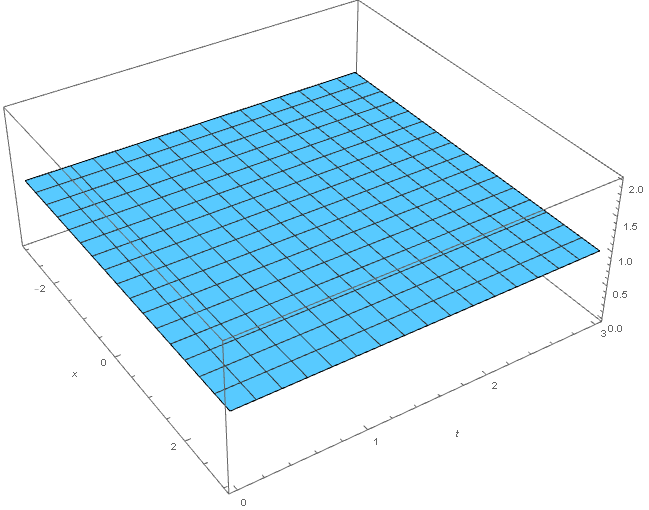
\includegraphics[width=\textwidth]{Part1Plots/plot2}
    \end{subfigure}
    \caption{Plot of $v_2(x,t)$ with $J_{2}(x,t)=1$} \label{fig:jext2}
\end{figure}


\pagebreak
\subsubsection{Example Function 3}
For $J_{3}(x,t) = \sin(x)$, the solution and plot is:
$$ v_3(x,t) = \frac{\sin(x)}{2} $$

\begin{figure}[H]
	\centering
	\begin{subfigure}[h]{0.8\textwidth}
        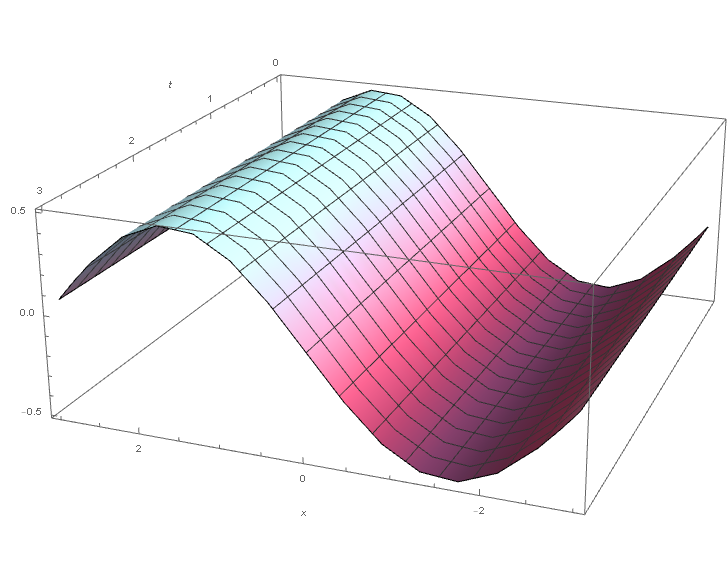
\includegraphics[width=\textwidth]{Part1Plots/plot3}
    \end{subfigure}
    \caption{Plot of $v_{3}(x,t)$ with $ J_3(x,t) = \frac{\sin(x)}{2} $ } \label{fig:jext3}
\end{figure}

\pagebreak

\subsection{Numerical Solutions}
After analytically solving the voltage equation, we also found numerical solutions. In order to numerically solve for this partial differential equation, we must first discretize both partial derivatives. For this problem, discretization is the process of using Taylor series to approximate the first time derivative of the voltage function in terms of the point we will approximate and the known point one time step before it, like so:
\[\frac{\partial{v(x,t)}}{\partial{t}}=\frac{v^{j+1}_i-v^j_i}{\Delta{t}}+O(\Delta{t})\]
In this equation, $v^j_i$ represents the point at $x=x_i$ and $t=t_j$ and $O(\Delta{t})$ represents the order of the error of this approximation, meaning that the error is a function of the size of the timestep.
Using the same approach, we will use Taylor series to write the second x derivative of the voltage function in terms of three known points, like so:
\[\frac{\partial^2{v(x,t)}}{\partial{x}^2}=\frac{v^{j}_{i+1}-2v^j_i+v^j_{i-1}}{(\Delta{x})^2}+O((\Delta{x})^2)\]
Using these two formulas and putting these into our original PDE gives:
\[\frac{v^{j+1}_i-v^j_i}{\Delta{t}}=\frac{v^{j}_{i+1}-2v^j_i+v^j_{i-1}}{(\Delta{x})^2}-v^j_i+J_{ext}(x,t)\]
Finally, we can algebraically solve this equation for $v^{j+1}_i$, in terms of values that are known. Therefore, going timestep by timestep starting from the initial condition, this question can be used to solve numerically for the entire subset of the neuron we're examining. Note that I have removed the $J_{ext}(x,t)$ from this equation
\begin{equation} \label{*}
v^{j+1}_i=\frac{\Delta{t}}{(\Delta{x})^2}(v^{j}_{i+1}+v^{j}_{i-1})+(1-\frac{\Delta{t}(2+(\Delta{x})^2)}{(\Delta{x})^2})v^{j}_{i}+\Delta{t}*J_{ext}(x,t)
\end {equation}
However, looking at the $v^{j}_{i}$ term in this equation, it can be seen that if $\frac{\Delta{t}(2+(\Delta{x})^2)}{(\Delta{x})^2}>1$ then this approximation is unstable and will not converge. Therefore, in order for this method of finite difference approximation to converge, $\Delta{t}$ must be much smaller than $\Delta{x}$. \par 
When using equation (\ref{*}) to approximate this solution numerically, we will be using $J_{ext}(x,t)=10e^{-25x^2}\delta{(t)}$. However, instead of simulating the function $\delta{(t})$, we will remove $J_{ext}(x,t)$ from the function representing the numerical function and use it as the initial condtion, making $v(x,0)=10e^{-25x^2}$. The boundary conditions will be zero everywhere else. Since we cannot approximate an infinite interval of x and t, we will instead look at the region from $[-10,10]$ for x and $[0,50]$ for t. 
First, using the given $\Delta{t}=0.1$ and $\Delta{x}=0.1$, we can see the the approximation does not converge to a solution, as predicted, and that it is unstable. 
\begin{figure}[H]
  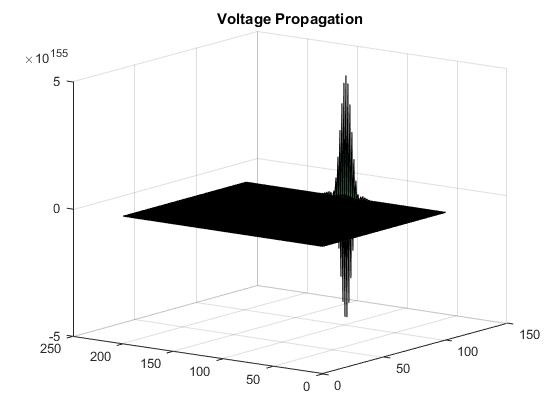
\includegraphics[width=\linewidth]{plot1.jpg}
  \caption{Plot of Unstable Numerical Approximation}
  \label{fig:sketch1}
\end{figure}
In this figure, we had to shorten the total time to 10 seconds because by time fifty, the instability caused parts of the solutions to approach infinity, so Matlab was not able to plot it reasonably. One can see in this plot that as time increases, the voltage increases exponentially higher than it began. \par
Next, when we change $\Delta{t}$ to 0.001 to meet the conditions for stability of this approximation, we can see that the approximation closely resembles our analytic solution to this partial differential equation.
\begin{figure}[H]
  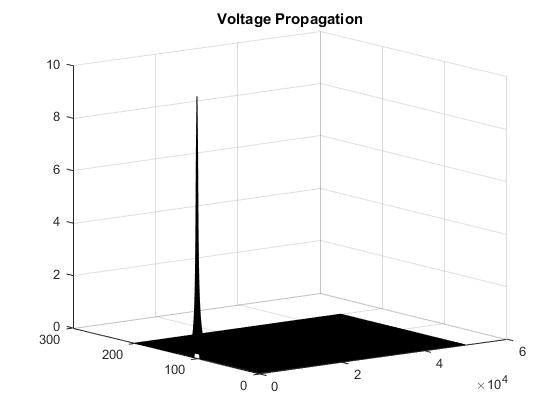
\includegraphics[width=\linewidth]{Plot2.jpg}
  \caption{Plot of Stable Numerical Approximation}
  \label{fig:sketch2}
\end{figure}
As one can see, this plot closely matches the analytical solution. It shows the spike of voltage at $t=0$ and $x=0$ and demonstrates how that voltage propagates throughout the neuron, approaching zero as time and x increases. \par
In order to make the propagation more apparent, I included the graph below, where each line indicates a different time step:
\begin{figure}[H]
  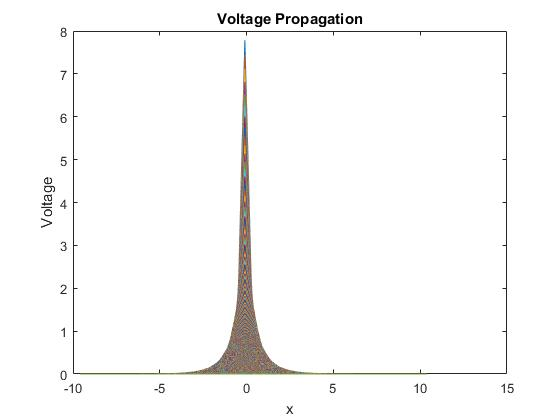
\includegraphics[width=\linewidth]{othergraph1.jpg}
  \caption{Plot of Stable Numerical Approximation}
  \label{fig:sketch2}
\end{figure}
Next, I displayed a plot of the voltages for only the times 25-50 seconds, to show the scaling on the remaining values. Although they appear to all be zero in the initial graph, they are nonzero and diminishing as one would expect with ions leaking out of the cell, as is the case in this scenario.
\begin{figure}[H]
  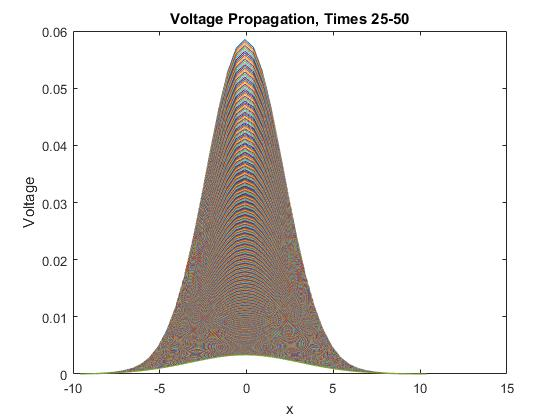
\includegraphics[width=\linewidth]{othergraph2.jpg}
  \caption{Plot of Stable Numerical Approximation, Times 25-50}
  \label{fig:sketch2}
\end{figure}

\section{Traveling Wave Solutions to the Cable Equation}
The local voltage of the neural membrane and the behavior of the ion currents depend on one another. One way to explore the effects of this dependency is to choose an ionic current $f(v(x,t))$ that results in a bistable system. In this context, bistable means the membrane has two stable equilibria described by an active and an inactive state. This bistable system yields traveling wave solutions to the cable equation. These two states can be implemented in the equation using the Heaviside step nonlinearity, which is defined to be $f(v)=-v+H(v-\theta)$.\\

\begin{equation}\label{generalHeaviside}
  H(v-\theta)=\begin{cases}
    0, & \text{when $v<\theta$}.\\
    1, & \text{when $v>\theta$}.
  \end{cases}
\end{equation}


\subsection{Homogeneous Solutions}
First, look for homogeneous solutions that are constant in both space and time, denoted $v(x,t)=\overline{v}$. The two possible homogeneous solutions of $\frac{\partial v(x,t)}{\partial t}=\frac{\partial ^2 v(x,t)}{\partial x^2}-v(x,t)+H(v-\theta)+J_{ext}(x,t)$ are found by taking the appropriate derivatives of $v(x,t)=\overline{v}$ and substituting them into the partial differential equation. 
$$\frac{\partial \overline{v}(x,t)}{\partial t}=0$$
$$\frac{\partial ^2 \overline{v}(x,t)}{\partial x^2}=0$$
$$0=0-\overline{v}+H(\overline{v}-\theta)$$
When $\overline{v}>\theta$, $0=-\overline{v}+1$. When $\overline{v}<\theta$, $0=-\overline{v}+0$

Thus, the two homogeneous solutions are 
$$\overline{v}^+=1\text{, when $\overline{v}>\theta$}$$
$$\overline{v}^-=0\text{, when $\overline{v}<\theta$}$$
In order for both of these solutions to exist, we require that $\theta\in(0,1)$. Consider $\overline{v}^+=1$. Equation (\ref{generalHeaviside}) is only satisfied when $1=H(1-\theta)$, which implies $1>\theta$. Now consider $\overline{v}^-=0$. Then $0=H(0-\theta)$ implies $0<\theta$.

\subsection{Change of Variables and Boundary Conditions}
Since the ratio of the diameter to the length of a neuronal axon is very small, we will impose the assumption that they are infinitely long cables with $x\in (-\infty,\infty)$. Furthermore, we will impose the following boundary conditions
$$\lim_{x\to\infty} \frac{\partial v(x,t)}{\partial x}=0 \text{ and } \lim_{x\to-\infty} \frac{\partial v(x,t)}{\partial x}=0.$$
Physically, these boundary conditions are significant because as x approaches the outer ends of the neurons, the voltage should not be changing. \par
In order to find traveling wave solutions, we can apply the change of variables $v(x,t)=V(\xi),$ where $\xi=x-ct$, to the partial differential equation. Furthermore, assume that the external current $J_{ext}(x,t)$ is $0$. The new second order ordinary differential equation is 
\begin{equation}
\label{second order ODE}
-cV'(\xi)=V''(\xi)-V(\xi)+H(V(\xi)-\theta)
\end{equation}

In order to solve for traveling wave solutions, we assume that the solution is a traveling front solution that decreases as $\xi$ increases. So, define $V(\xi)>\theta$ when $\xi<0$ and that $V(\xi)<\theta$ when $\xi>0$. The Heaviside step nonlinearity is now defined as 

\begin{equation}
  H(V(\xi)-\theta)=\begin{cases}
    0, & \text{when $V(\xi)<\theta$}.\\
    1, & \text{when $V(\xi)>\theta$}.
  \end{cases}
\end{equation}

Equation (\ref{second order ODE}) can now be decomposed into the following two second order ordinary differential equations for $V_1(\xi)$ and $V_2(\xi)$.
\begin{equation}
\label{ODE1}
-cV_1'(\xi)=V_1''(\xi)-V_1(\xi) \text{ when  $\xi \in (0,\infty)$}
\end{equation}

\begin{equation}
\label{ODE2} 
-cV_2'(\xi)=V_2''(\xi)-V_2(\xi)+1 \text{ when $\xi \in (-\infty,0)$.}
\end{equation}

In order to ensure the solutions to equations (\ref{ODE1}) and (\ref{ODE2}) are physically realistic, we must impose boundary conditions. $V(\xi)$ must approach the homogeneous solution as $\xi$ approaches $\pm \infty$. Also, the two solutions and their first derivatives must match at $\xi=0$. Physically, this is because we want to model the voltage, which should be differentiable. The boundary conditions are:\\
$$\lim_{\xi\to-\infty} \frac{d V_1(\xi)}{d \xi}=0$$
$$\lim_{\xi\to\infty} \frac{d V_2(\xi)}{d \xi}=0$$
$$\lim_{\xi\to-\infty} V_1(\xi)=1$$
$$\lim_{\xi\to\infty} V_2(\xi)=0$$
$$V_1(0)=V_2(0)$$
$$\frac{d V_1}{d \xi}(0)=\frac{d V_2}{d \xi}(0)$$


\subsection{Solving for Traveling Wave Solutions}

Equation (\ref{ODE1}) is a homogeneous ordinary differential equation. The corresponding characteristic equation, $r^2+cr-1=0$, has roots of  $r=\frac{-c \pm \sqrt{c^2+4}}{2}$. The general solution to equation (\ref{ODE1}) is 
\begin{equation}
\label{ODE1 general solution}
V_{1}=c_1 e^{\frac{1}{2}(-c+\sqrt{c^2+4})\xi}+c_2e^{-\frac{1}{2}(c+\sqrt{c^2+4})\xi}, \quad \xi \in (0,\infty)
\end{equation}

Equation (\ref{ODE2}) is not homogeneous, but can be solved using the method of undetermined coefficients. First, the homogeneous solution is obtained by solving $cV_2'(\xi)=V_2''(\xi)-V_2(\xi)$ for $V_2$. The homogeneous solution is
$$V_{2,h}=c_3 e^{\frac{1}{2}(-c+\sqrt{c^2+4})\xi}+c_4 e^{-\frac{1}{2}(c+\sqrt{c^2+4})\xi}$$
Now, we guess a particular solution of the form $V_{2,p}=A$. Plugging $V_{2,p}$ into equation (\ref{ODE2}) yields 
$$-c(0)=0-A+1$$
$$A=1$$ 
$$V_{2,p}=1$$
Thus, the solution to equation (\ref{ODE2}) is 
\begin{equation}
\label{ODE2 general solution}
V_{2}=c_3 e^{\frac{1}{2}(-c+\sqrt{c^2+4})\xi}+c_4 e^{-\frac{1}{2}(c+\sqrt{c^2+4})\xi}+1, \quad \xi \in (-\infty,0)
\end{equation}
Next, use the boundary conditions to eliminate the unknown coefficients from equations (\ref{ODE1 general solution}) and (\ref{ODE2 general solution}). 
$$\lim_{\xi\to\infty} \frac{d V_1(\xi)}{d \xi}=0\Rightarrow c_1=0$$
$$\lim_{\xi\to-\infty} \frac{d V_2(\xi)}{d \xi}=0\Rightarrow c_4=0$$
$$V_1(0)=V_2(0)\Rightarrow c_2=c_3+1$$
$$\frac{d V_1}{d \xi}(0)=\frac{d V_2}{d \xi}(0)\Rightarrow -\frac{1}{2}(c+\sqrt{c^2+4}) c_2= \frac{1}{2}(-c+\sqrt{c^2+4})c_3$$ 
The solution to this linear system of equations is $c_1=0, c_2=\frac{-c+\sqrt{c^2+4}}{2\sqrt{c^2+4}}, c_3=\frac{-c-\sqrt{c^2+4}}{2\sqrt{c^2+4}}$, and $c_4=0$. So, the solution to equation (\ref{ODE1}) is 
\begin{equation}
\label{ODE1 solution}
V_1(\xi)=\frac{-c+\sqrt{c^2+4}}{2\sqrt{c^2+4}}e^{-\frac{1}{2}(c+\sqrt{c^2+4})\xi},\quad \xi \in (0,\infty).
\end{equation}
The solution to equation (\ref{ODE2}) is
\begin{equation}
\label{ODE2 solution}
V_2(\xi)=\frac{-c-\sqrt{c^2+4}}{2\sqrt{c^2+4}}e^{\frac{1}{2}(-c+\sqrt{c^2+4})\xi}+1,\quad \xi \in (-\infty,0).
\end{equation}
\begin{figure}[H]
\centering
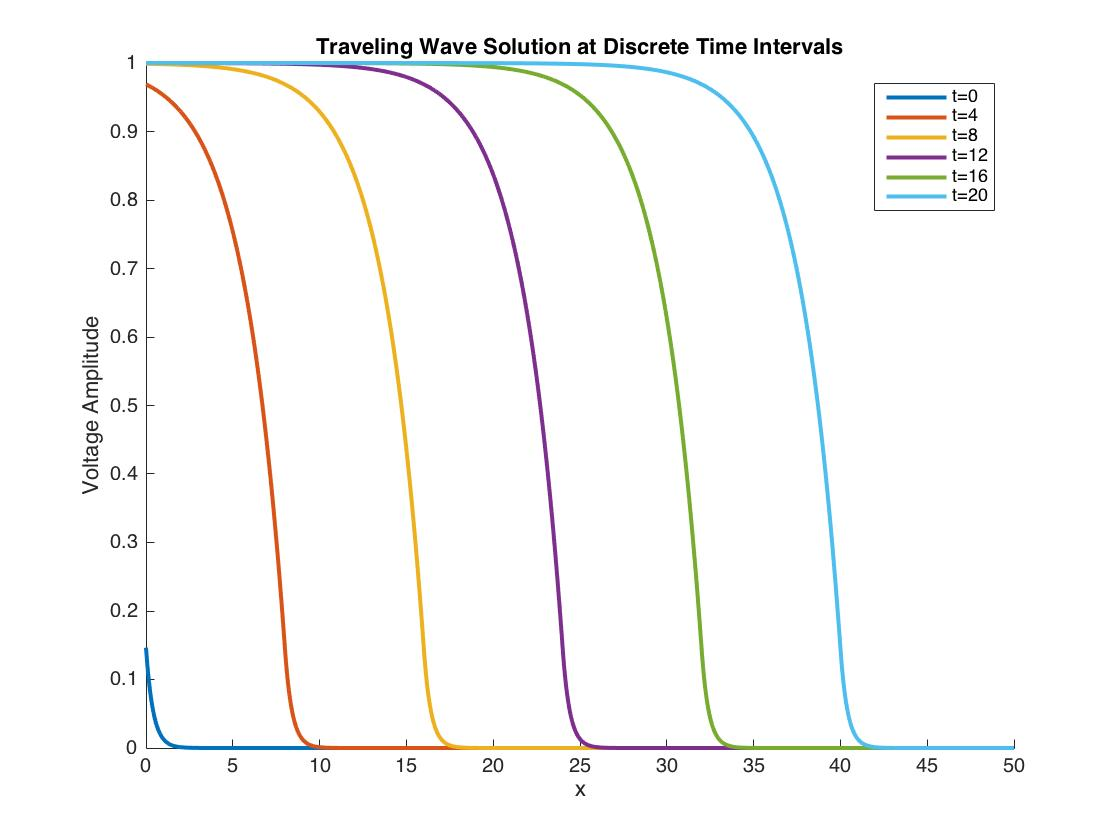
\includegraphics[width=0.7\textwidth]{waveThang.jpg}
\caption{Traveling Wave Solution at Discrete Time Intervals}
\label{kahkaw}
\end{figure}

The figure above shows the voltage of the traveling wave solution as a function of space at discrete intervals of time. As time elapses, the "wave" moves to the right. 


\subsection{Analysis of the Traveling Wave Solution}
In order to understand the relationship between the speed of the traveling front, c, and the threshold value, $\theta$, apply the threshold condition that $V(0)=\theta$. Application of this threshold condition to the traveling wave solutions gives $\frac{-c}{2\sqrt{c^2+4}}+\frac{1}{2}=\theta$. Now, we will solve this equation for $c$. 
$$c=\sqrt{\frac{-(2\theta-1)^2}{\theta^2-\theta}}$$

\begin{figure}[H]
\centering
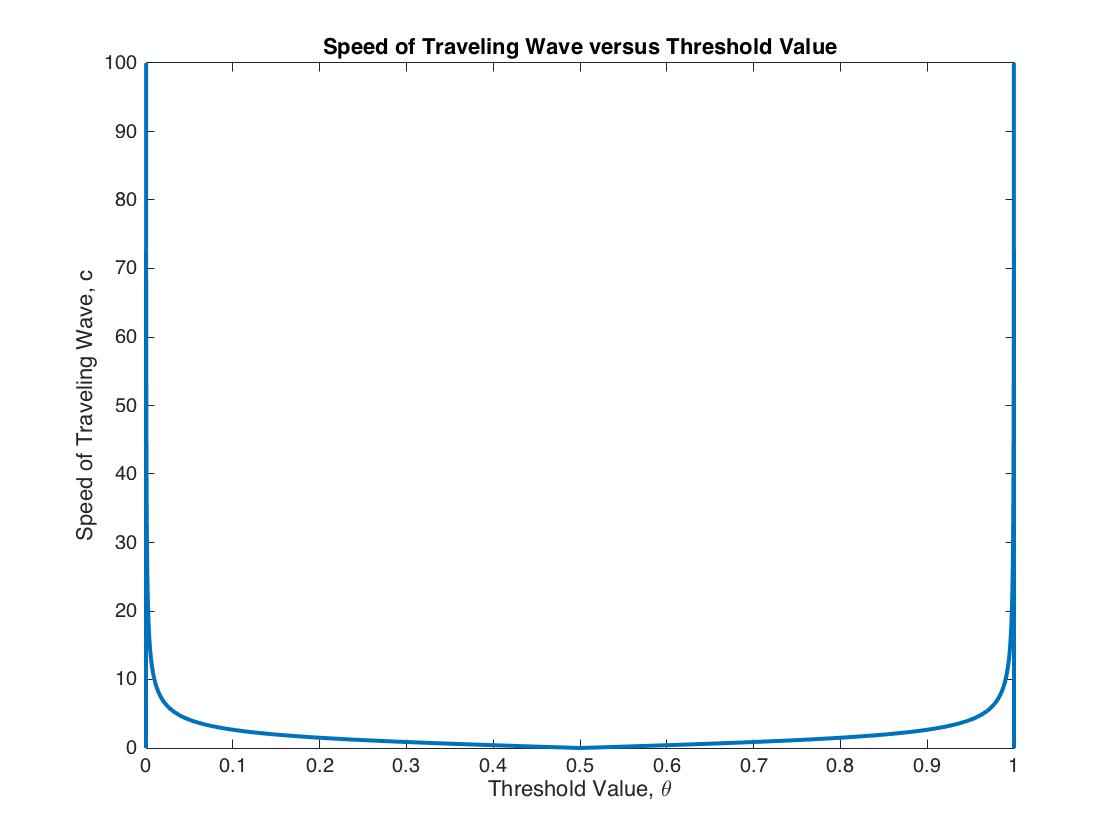
\includegraphics[width=0.7\textwidth]{cVStheta.jpg}
\caption{Speed of Traveling Wave vs. Threshold Value}
\label{test}
\end{figure}

Figure (\ref{test}) above demonstrates that as $\theta \rightarrow 0$, then $c \rightarrow \infty$, and as $\theta \rightarrow 1$, then $c \rightarrow \infty$ as well. This makes sense because we know that $V(0)=\theta$, and the original equation is modeling a bistable system with two stable equilibria at $v=0$ and $v=1$. Therefore, if $\theta$ is close to either 0 or 1, it makes sense that it will be drawn towards its nearest stable state at a faster speed. Alternatively, if $\theta=0.5$, it will have a speed $c=0$ because it is drawn equally to both stable states and thereby forced to remain stagnant. 

\subsection{Stability of the Traveling Front Solutions}
Now that we have found the traveling front solutions, it is important to understand their stability using linear stability analysis. Consider the solution $v(x,t)=V(\xi)+\epsilon\psi(\xi,t)$, where $0 < \epsilon <<1$ and $\psi(\xi,t)$ represents a small perturbation to the traveling wave solution, $V(\xi)$. The goal of the linear stability analysis is to understand how $\psi(\xi,t)$ behaves over time. Recall the governing partial differential equation
\begin{equation}
\label{uh}
\frac{\partial v}{\partial t}=\frac{\partial ^2 v}{\partial x^2}-v+H(v-\theta)
\end{equation}
\\
The chain rule allows us to obtain the following partial derivatives of $v(x,t)=V(\xi)+\epsilon\psi(\xi,t)$.

$$\frac{\partial v}{\partial t}=\frac{\partial\xi}{\partial t}\frac{dV}{d\xi}+\epsilon(\frac{\partial \psi}{\partial \xi}\frac{\partial \xi}{\partial t}+\frac{\partial \psi}{\partial t}) = -c\frac{dV}{d\xi}+\epsilon(-c\frac{\partial \psi}{\partial \xi}+\frac{\partial \psi}{\partial t})$$

$$\frac{\partial v}{\partial x}=\frac{\partial \xi}{\partial x}\frac{dV}{d\xi}+\epsilon\frac{\partial\xi}{\partial x}\frac{\partial\psi}{\partial\xi} = \frac{dV}{d\xi}+\epsilon\frac{\partial\psi}{\partial\xi}$$

$$\frac{\partial^2 v}{\partial x^2}=\frac{\partial \xi}{\partial x}\frac{d^2V}{d\xi^2}+\epsilon\frac{\partial^2\psi}{\partial\xi^2}\frac{\partial \xi}{\partial x} = \frac{d^2V}{d\xi^2}+\epsilon\frac{\partial^2\psi}{\partial\xi^2}$$
Equation (\ref{uh}) is rewritten as 
\begin{equation}
\label{frewritten}
-c\frac{dV(\xi)}{d\xi}+\epsilon(-c\frac{\partial \psi(\xi,t)}{\partial \xi}+\frac{\partial \psi(\xi,t)}{\partial t})=\frac{d^2V(\xi)}{d\xi^2}+\epsilon\frac{\partial^2\psi(\xi,t)}{\partial\xi^2}+f(V(\xi)+\epsilon\psi(\xi,t))
\end{equation}
Analysis of equation (\ref{frewritten}) can be simplified by using the Taylor expansion of $f\big(V(\xi)+\epsilon\psi(\xi,t)\big)$ with respect to $V(\xi)$, and discounting $O(\epsilon ^2)$ terms.

$$f\big(V+\epsilon\psi \big) \approx f(V) + \frac{\partial f(V)}{\partial V}\epsilon\psi = -V +\mathcal{H}(V-\theta) - \epsilon\psi + \delta(V-\theta)\epsilon\psi $$
Equation \ref{frewritten} becomes
$$-c\frac{dV}{d\xi}+\epsilon(-c\frac{\partial \psi}{\partial \xi}+\frac{\partial \psi}{\partial t})= 
\frac{d^2V}{d\xi^2}+\epsilon\frac{\partial^2\psi}{\partial\xi^2}-V+H(V-\theta)+\epsilon\psi\big(-1+\delta(V-\theta)\big)$$
Look at the terms involving $\psi$ and $\epsilon$ to analyze the long term behavior of the disturbance. The partial differential equation that models the behavior of the perturbation is

\begin{equation} \label{pde_nh}
\frac{\partial \psi}{\partial t} = c \frac{\partial^2\psi}{\partial\xi^2} + \frac{\partial\psi}{\partial\xi} - (1 - \delta(V-\theta))\psi
\end{equation} 


\subsection{Separation of Variables}

This equation can be solved using separation of variables, where solutions have the form of $\psi(\xi,t)=S(\xi)T(t)\neq0$.

$$ \frac{1}{T}\frac{\partial T}{\partial t} = \frac{1}{S}\frac{\partial^2S}{\partial\xi^2} + \frac{c}{S}\frac{\partial S}{\partial\xi} - 1 + \delta(V-\theta)= \lambda $$
Before proceeding with the analysis, we need to define the boundary conditions. Recall that the boundary condition $\lim_{x\to\pm\infty} \frac{\partial v(x,t)}{\partial x}=0$ is necessary to ensure a physically realistic solution. Because we previously imposed the boundary condition that $\lim_{\xi\to\pm\infty} \frac{dV}{d\xi}=0$, it must also be true that 

$$\lim_{x\to\pm\infty} \frac{\partial \big(V(\xi)+\epsilon\psi(\xi,t)\big)}{\partial x} = \lim_{\xi\to\pm\infty} \frac{dV}{d\xi}+\lim_{\xi\to\pm\infty} \epsilon\frac{\partial\psi}{\partial\xi}=0 \implies \lim_{\xi\to\pm\infty}\frac{d\psi}{d\xi}=0 $$
The time-dependent equation is a homogeneous ODE with the following solutions, where $a\in\mathbb{R}$.
\begin{equation} \label{timeeq}
\frac{1}{T}\frac{dT}{dt} = \lambda \implies \int\frac{dT}{T} = \int\lambda dt \implies T(t)=ae^{\lambda t}
\end{equation}
For the spatial dependence, we split the domain of the equation into three regions, depending on the value of $\delta(V(\xi)-\theta)$, with the boundary condition that $\lim_{\xi \to \pm \infty}\psi = 0$:

Region 1: $\xi < 0$ and $\delta(V(\xi)-\theta) = 0$

Region 2: $\xi > 0$ and $\delta(V(\xi)-\theta) = 0$ 

Region 3: $\xi = 0$ and $\delta(V(\xi)-\theta) = \infty$

\subsubsection{ Region 1 and 2}
In Region 1 and 2, we solve the equation:

\begin{equation}
\frac{d^2S}{d\xi^2} + c\frac{dS}{d\xi} - (\lambda + 1)S = 0
\end{equation} 
The boundary conditions are in Region 1: $\lim_{\xi \to -\infty}S_1 = 0$; and in Region 2: $\lim_{\xi \to \infty}S_2 = 0$. The solutions have the form:

\begin{equation} \label{homogsln}
\begin{aligned}
S_1(\xi) = c_1e^{\frac{-c+\sqrt{c^2+4(\lambda+1)}}{2}\xi} \\
S_2(\xi) = c_2e^{\frac{-c-\sqrt{c^2+4(\lambda+1)}}{2}\xi} 
\end{aligned}
\end{equation}

\subsubsection{Region 3}
At Region 3, we integrate the equation at a small interval around the point of discontinuity to examine the effect $\delta(V(\xi)-\theta)$ has on the solution. The spatial equation in this region is 

\begin{equation}
\frac{d^2S}{d\xi^2} + c\frac{dS}{d\xi} - \big[\lambda + 1 + \delta(V(\xi)-\theta)\big]S = 0
\end{equation} 
Since there is a discontinuity due to the dirac delta function here at $V(\xi) = \theta$, $\xi = 0$, we integrate a small interval $(+\epsilon,-\epsilon)$ around the discontinuity. The limit $\epsilon \to 0$ gives us information as to how the solutions in Region 1 and 2, (\ref{homogsln}), connect in Region 3.

$$ \int_{-\epsilon}^{+\epsilon}\frac{d^2S}{d\xi^2}d\xi + c\int_{-\epsilon}^{+\epsilon}\frac{dS}{d\xi}d\xi - \int_{-\epsilon}^{+\epsilon}(\lambda + 1)Sd\xi - \int_{-\epsilon}^{+\epsilon}\delta(V(\xi)-\theta)Sd\xi = 0 $$
For the first two terms, the fundamental theorem of calculus gives us the first derivative evaluated at the endpoints and the function evaluated at the endpoints.
$$ \frac{dS}{d\xi}(+\epsilon) - \frac{dS}{d\xi}(-\epsilon) + c[S(+\epsilon) - S(-\epsilon)] - \int_{-\epsilon}^{+\epsilon}(\lambda + 1)Sd\xi - \int_{-\epsilon}^{+\epsilon}\delta(V(\xi)-\theta)Sd\xi = 0 $$
Now we take the limit:
$$ \lim_{\xi \to 0} \Bigg[ \frac{dS}{d\xi}(+\epsilon) - \frac{dS}{d\xi}(-\epsilon) + c[S(+\epsilon) - S(-\epsilon)] - \int_{-\epsilon}^{+\epsilon}(\lambda + 1)Sd\xi - \int_{-\epsilon}^{+\epsilon}\delta(V(\xi)-\theta)Sd\xi \Bigg]= 0 $$
Of the remaining two integrals, the first one goes to zero as the bounds shrink to zero since the integral is continuous, even if $S$ is not. The second integral involving the dirac delta function evaluates to $S(0)$ by the \textit{sampling property}, since we are specifically looking at the small region centered around where $V(\xi) = \theta$. Therefore we get:
$$ \lim_{\xi \to 0} \Bigg[ \frac{dS}{d\xi}(+\epsilon) - \frac{dS}{d\xi}(-\epsilon) + c[S(+\epsilon) - S(-\epsilon)] \Bigg] = S(0) $$
$S$ must be continuous if we are assuming that the derivative $\frac{dS}{d\xi}$ exists so $S(0^+) = S(0^-)$ and the constants in front of the homogeneous solutions (\ref{homogsln}) are equal, $c_1 = c_2 = K$ (using $K$ to avoid confusion with the speed $c$), revealing a relationship between the value of the spatial term and the discontinuity between its derivative at $\xi=0$.
$$ S(0) = \lim_{\xi \to 0} \Bigg[ K(\frac{-c-\sqrt{c^2+4(\lambda+1)}}{2}e^{\frac{-c-\sqrt{c^2+4(\lambda+1)}}{2}\xi} - \frac{-c+\sqrt{c^2+4(\lambda+1)}}{2}e^{\frac{-c+\sqrt{c^2+4(\lambda+1)}}{2}\xi})\Bigg] $$
Taking the limit, we find the following, where $S(0)\in \mathbb{R}$ and $K\in\mathbb{R}$ since this is a physical system and we assume the solutions are real-valued.
\begin{equation}\label{Keq}
S(0) = K\Bigg(\frac{-c-\sqrt{c^2+4(\lambda+1)}}{2} - \frac{-c+\sqrt{c^2+4(\lambda+1)}}{2} \Bigg)
\end{equation}
$S$ is the spatial part of some arbitrary perturbation function that satisfies $\lim_{\xi \to \pm \infty}S(\xi) = 0$, and its value at zero could be either non-zero, or it could be 0. Since the boundary conditions provided do not fix $S(0)$ or $K$, we will examine both cases. In the latter case, if $S(0) = 0$ then $K=c_1=0$ and we find the trivial solution of $S=0$ which gives us $\psi(\xi,t) = 0$. In the following section, we explore the former case.


\subsection{Eigenvalues}
\subsubsection{$\lambda = 0$ Case}
Now to examine the family of solutions that depend on $\lambda$, we start with the $\lambda = 0$ case. Assuming we can rescale $S(0)$ to unity, eq (\ref{Keq}) simplifies to:
$$1 = K\Bigg(\frac{-c-\sqrt{c^2+4)}}{2} - \frac{-c+\sqrt{c^2+4)}}{2}\Bigg) = -K\sqrt{c^2+4} $$
or
$$K = -\frac{1}{\sqrt{c^2+4}}$$
Plugging this constant back into our solutions for Region 1 and 2 (\ref{homogsln}) and multiplying it by the time-dependent solution (\ref{timeeq}), we find a solution for $\psi(\xi,t)$:

\begin{equation}\label{solnlambda0}
\psi_{\lambda=0}(\xi,t)=
\begin{cases}
\ \frac{-1}{\sqrt{c^2+4}}e^{\frac{-c+\sqrt{c^2+4}}{2}\xi},\quad \xi < 0 \\
\ \frac{-1}{\sqrt{c^2+4}}e^{\frac{-c-\sqrt{c^2+4}}{2}\xi},\quad \xi > 0\\
\end{cases}
\end{equation}
Recalling our traveling wave solution $V(\xi)$ (\ref{ODE2 solution}), we note that $\psi(\xi,t) = V'(\xi)$. This solution corresponds to $v(x,t) = V(\xi) + \epsilon V'(\xi)$, a Taylor expansion linearization around the traveling wave solution. This perturbation is independent of time. We plot $v(x,t)$ with various values of $\epsilon$ to show its effect on $V(\xi)$.

\begin{figure}[H]
    \centering
    \begin{subfigure}[h]{0.4\textwidth}
        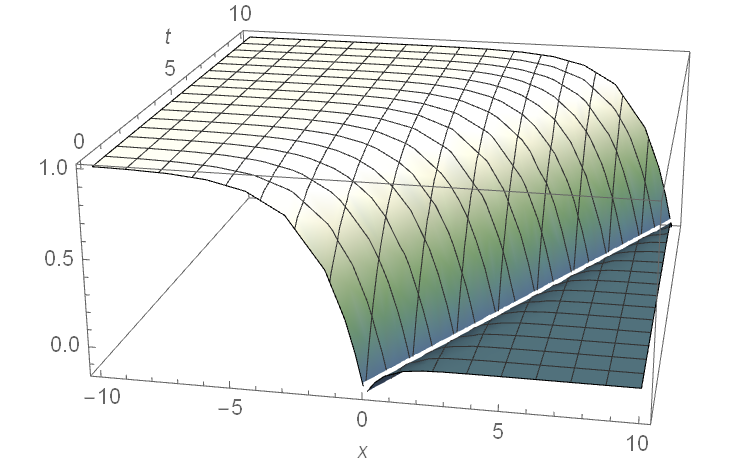
\includegraphics[width=\textwidth]{Part2Plots/e099}
        \caption{$\epsilon=0.99$}
        \label{fig:e099}
    \end{subfigure}
    \begin{subfigure}[h]{0.4\textwidth}
        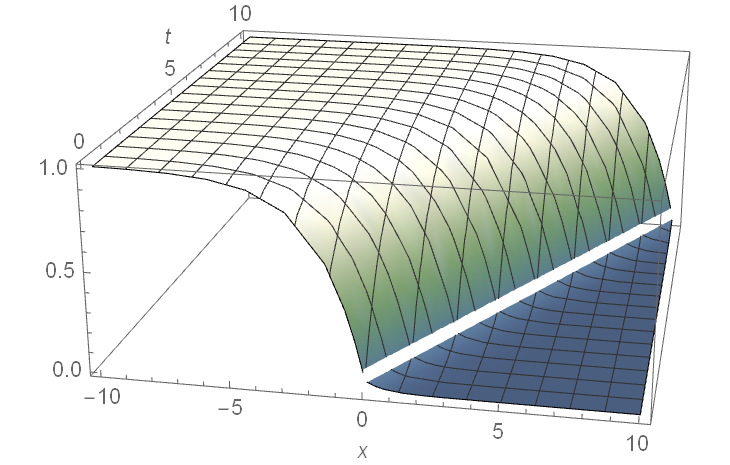
\includegraphics[width=\textwidth]{Part2Plots/e05}
        \caption{$\epsilon=0.5$}
        \label{fig:e05}
    \end{subfigure}
    \begin{subfigure}[h]{0.4\textwidth}
        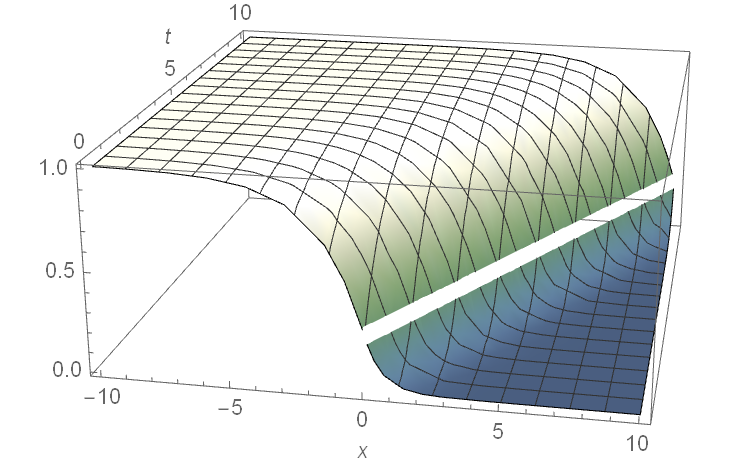
\includegraphics[width=\textwidth]{Part2Plots/e001}
        \caption{$\epsilon=0.01$}
        \label{fig:t10}
    \end{subfigure}
    \begin{subfigure}[h]{0.4\textwidth}
        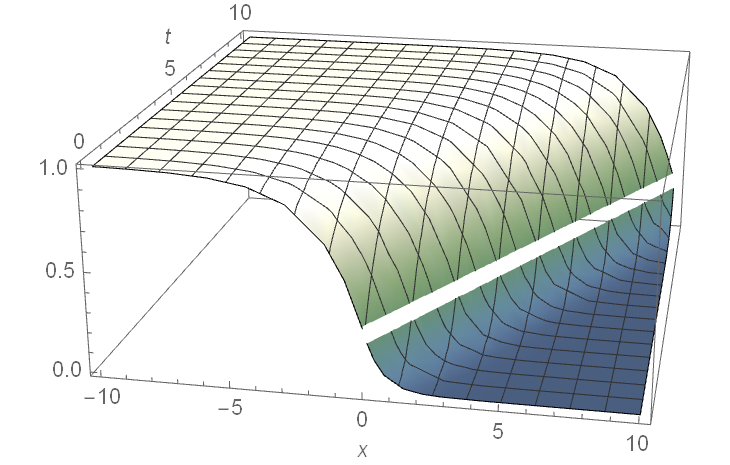
\includegraphics[width=\textwidth]{Part2Plots/e0}
        \caption{$\epsilon=0$}
        \label{fig:e0}
    \end{subfigure}
    \caption{$v(x,t) = V(\xi) + \epsilon V'(\xi)$ with various $\epsilon$ values}\label{fig:epsilonplots}
\end{figure}

While this perturbation is independent of time, $v(x,t)$ actually solves the original ODE for the traveling wave solution (\ref{second order ODE}). Therefore, it is another traveling wave solution.

\subsubsection{$\lambda \neq 0$ Case}
Looking at this case, we revert back to using $S(0)$ as a parameter and combine it with the time-dependent solutions in eq(\ref{timeeq}),we find  solutions of the form.
\begin{equation}\label{solnlambda+}
\psi_{\lambda >0}(\xi,t)=
\begin{cases}
\ \frac{-S(0)}{\sqrt{c^2+4(\lambda+1)}}e^{\frac{-c+\sqrt{c^2+4(\lambda+1)}}{2}\xi+\lambda t},\quad \xi < 0 \\
\ \frac{-S(0)}{\sqrt{c^2+4(\lambda+1)}}e^{\frac{-c-\sqrt{c^2+4(\lambda+1)}}{2}\xi+\lambda t},\quad \xi > 0\\
\end{cases}
\end{equation}
The derivatives are given by:
\begin{equation}\label{solndevlambda+}
\partial_{\xi} \psi_{\lambda >0}(\xi,t)=
\begin{cases}
\ \frac{-S(0)}{2}e^{\frac{-c+\sqrt{c^2+4(\lambda+1)}}{2}\xi+\lambda t},\quad \xi < 0 \\
\ \frac{S(0)}{2}e^{\frac{-c-\sqrt{c^2+4(\lambda+1)}}{2}\xi+\lambda t},\quad \xi > 0\\
\end{cases}
\end{equation}
For $\lambda < 0$, we pull out the negative to find solutions of the form:

\begin{equation}\label{solnlambda-}
\psi_{\lambda <0}(\xi,t)=
\begin{cases}
\ \frac{-S(0)}{\sqrt{c^2-4(\lambda-1)}}e^{\frac{-c+\sqrt{c^2-4(\lambda-1)}}{2}\xi -\lambda t},\quad \xi < 0 \\
\ \frac{-S(0)}{\sqrt{c^2-4(\lambda-1)}}e^{\frac{-c-\sqrt{c^2-4(\lambda-1)}}{2}\xi-\lambda t},\quad \xi > 0\\
\end{cases}
\end{equation}

\begin{equation}\label{solndevlambda-}
\partial_{\xi}\psi_{\lambda <0}(\xi,t)=
\begin{cases}
\ \frac{-S(0)}{2}e^{\frac{-c+\sqrt{c^2-4(\lambda-1)}}{2}\xi -\lambda t},\quad \xi < 0 \\
\ \frac{S(0)}{2}e^{\frac{-c-\sqrt{c^2-4(\lambda-1)}}{2}\xi-\lambda t},\quad \xi > 0\\
\end{cases}
\end{equation}

We note that if $c^2-4(\lambda-1) < 0$  then the solutions will be complex. Without further boundary conditions, it is difficult to see what the difference between these two families of solutions are and why solutions with $\lambda > 0$ are not valid. 






\subsection{Numerical Solutions: Two-State Ion Channels}
After analytically solving the traveling wave solutions of the voltage equation, we found numerical solutions as well. In this case, the equation we examined was:
\[\frac{\partial{v(x,t)}}{\partial{t}}=\frac{\partial^2{v(x,t)}}{\partial{x}^2}-v(x,t)+H(v(x,t)-\theta)+J_{ext}(x,t)\]
Though the term $J_{ext}(x,t)$ was not specified, I will use $J_{ext}(x,t)=10e^{25x^2}\delta(t)$. This is the same $J_{ext}(x,t)$ used in numerically solving the passive membrane solution, and it can be removed from the equation itself and substituted into the initial condition. It mimics the scenario of a large spike of voltage initially applied to the neuron at $x=0$ and $t=0$, while remaining almost zero for all other $x$ at $t=0$. Also, though there are infinite boundaries for both $x$ and $t$, we will again only look at the region from $[-10,10]$ for x and $[0,50]$ for t in order to numerically solve this system.  Similar to the numerical solutions of the passive membrane, we will solve the system numerically by discretizing both partial derivatives using Taylor series, plugging these approximations back into the original partial differential equation, and solving for $v^{j+1}_i$. This gives the equation:
\begin{equation} \label{**}
v^{j+1}_i=\frac{\Delta{t}}{(\Delta{x})^2}(v^{j}_{i+1}+v^{j}_{i-1})+(1-\frac{\Delta{t}(2+(\Delta{x})^2)}{(\Delta{x})^2})v^{j}_{i}+\Delta{t}*H(v^j_i-\theta)
\end {equation}
This equation requires the same stability condition as the numerical approximation for the passive membrane solution. If $\frac{\Delta{t}(2+(\Delta{x})^2)}{(\Delta{x})^2}>1$ then this approximation is unstable and will not converge. Therefore, $\Delta{t}$ must be much smaller than $\Delta{x}$. This instability is demonstrated when we use the given values of $\Delta{x}=0.1$ and $\Delta{t}=0.1$. 
\begin{figure}[H]
  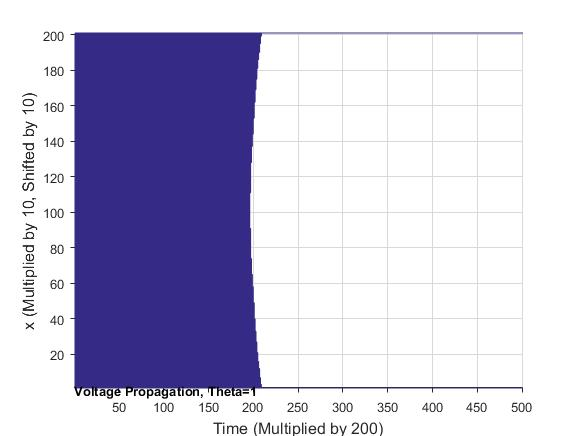
\includegraphics[width=\linewidth]{badplot3.jpg}
  \caption{Plot of Unstable Numerical Approximation, Two-State Ion Channel Solution}
  \label{fig:sketch3}
\end{figure}
Matlab was unable to plot this completely, because the divergence caused some of the points to not be able to compute. Therefore, for the rest of the problem, we will make $\Delta{x}=0.5$ and $\Delta{t}=0.005$. Next, we will produce plots of numerical solutions with three different values of $\theta$. The values we examined were $\theta=1$, $\theta=0.5$, $\theta=0.1$. 
\begin{figure}[H]
  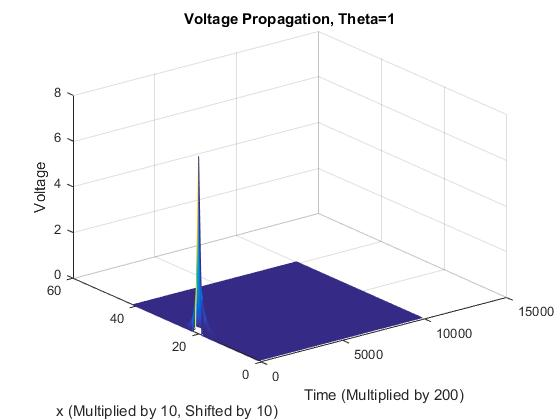
\includegraphics[width=\linewidth]{thetaone.jpg}
  \caption{Plot of Stable Numerical Approximation, Two-State Ion Channel Solution, $\theta=1$}
  \label{fig:sketch4}
\end{figure}
With this value of $\theta$ the plot doesn't look much different from the plots in the passive membrane solution. This is because when $\theta$ is large, not many of values of voltage, $v(x,t)$ will be greater than $\theta$ so the Heaviside function will be zero for most of the solution. Since this value of $\theta$ doesn't produce a traveling wave, we cannot numerically calculate the speed of the wave. 
\begin{figure}[H]
  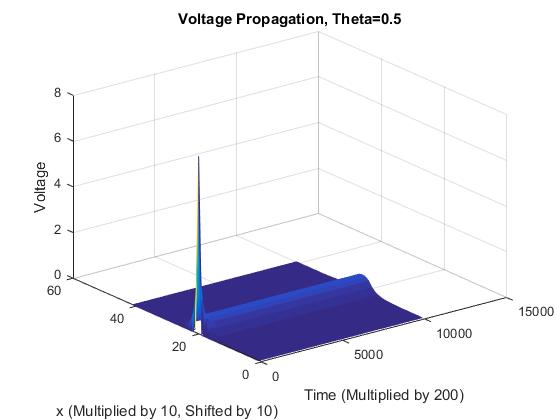
\includegraphics[width=\linewidth]{thetatwo.jpg}
  \caption{Plot of Stable Numerical Approximation, Two-State Ion Channel Solution, $\theta=0.5$}
  \label{fig:sketch5}
\end{figure}
With this value of $\theta$, there is a single wave of voltage, but its speed is zero. By exmining the graph, one can see that it converges to relatively constant position as time increases.This is verified for plugging in $\theta=1$ to the analytical equation for wave speed as a function of $\theta$ we found earlier in the report. As time increases, the solution converges to a uniform wave that doesn't change shape and remains stationary throughout time.
\begin{figure}[H]
  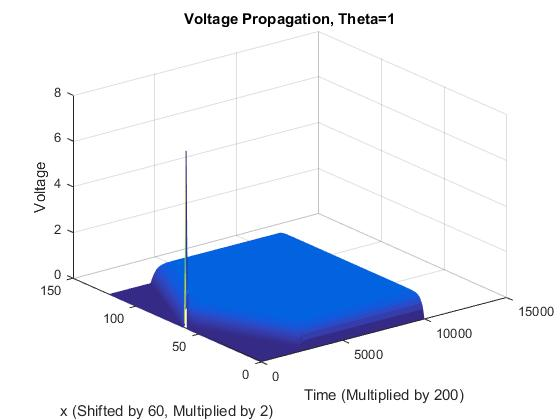
\includegraphics[width=\linewidth]{thetathree.jpg}
  \caption{Plot of Stable Numerical Approximation, Two-State Ion Channel Solution, $\theta=0.1$}
  \label{fig:sketch6}
\end{figure}
We found that for this value of $\theta$, the traveling wave front was better depicted with a wider range of x values, so x will go between $[-30,30]$ in this plot. One can see that initially, the wave is spreading from the center $x=0$ to the edges of the boundary. In an infinite boundary, this wave would spread throughout the entire neuron. \par
In order to approximate the speed of this wave numerically, we found the time at which a certain value of x reached a voltage above a certain threshold, and then we found the time that a different value of x (farther from the origin than the initial x value) reached a voltage above the same threshold. In this case, we used Matlab to find the first time that $x=80$ reached a voltage greater than or equal to $0.999$ and found the first time that $x=100$ reached this same value. By dividing the difference of these times by the distance of these x values, we were able to approximate that the wave was traveling at a speed of $c=2.27$ units of distance per units of time. \par
Earlier in the analytical solutions of the traveling wave solution, we found an equation that solves analytically for the speed of the wave with respect to $\theta$. When $\theta=0.1$, using this equation to solve for the speed analytically gives a value of $c=2.67$ units of distance per units of time. Therefore, our numerical solution is reasonably close to the analytical solution, especially considering that the highest error term in the equations using discretization to approximate the partial derivatives was of $O(\Delta{x})$, which in this case, $\Delta{x}=0.5$. Therefore, the error in the numerical approximation is within the given range of error. 




\subsubsection{Periodically Varying Threshold}
Now, we will find numerical solutions for a periodically varying threshold. This will be represented in our model by substituting in the following for $f(v(x,t))$:
\[f(v,x)=-v+H(v-\theta(1+0.5\cos(x)))\]
However, since we will want to examine the effects of different coefficients in front of the $\cos(x)$ term, I will label this coefficient $C$. The same steps are applied in order to find numerical solutions, where we discretize the parital derivatives and solve in terms of the value at the next timestep. Since this $f(v(x,t))$ is similar to the one in the previous model that we solved numerically for, the numerical approximation will look similar. It is shown below. 
\begin{equation} \label{***}
v^{j+1}_i=\frac{\Delta{t}}{(\Delta{x})^2}(v^{j}_{i+1}+v^{j}_{i-1})+(1-\frac{\Delta{t}(2+(\Delta{x})^2)}{(\Delta{x})^2})v^{j}_{i}+\Delta{t}*H(v^j_i-\theta(1+C\cos(x)))
\end {equation}
In order to analyze the numerical solutions, we used the three different values of $\theta$ from the numerical solution of the previous model, $\theta=1$, $\theta=0.5$, and $\theta=0.1$. For each of these three $\theta$ values, we used four different values of $C$, the constant preceding the $\cos(x)$ term. The first of which was the given value, 0.5, and the rest were $C=20$, $C=2$, and $C=-1$. All of these plots are shown below, grouped together by $\theta$ value
\begin{figure}[H]
  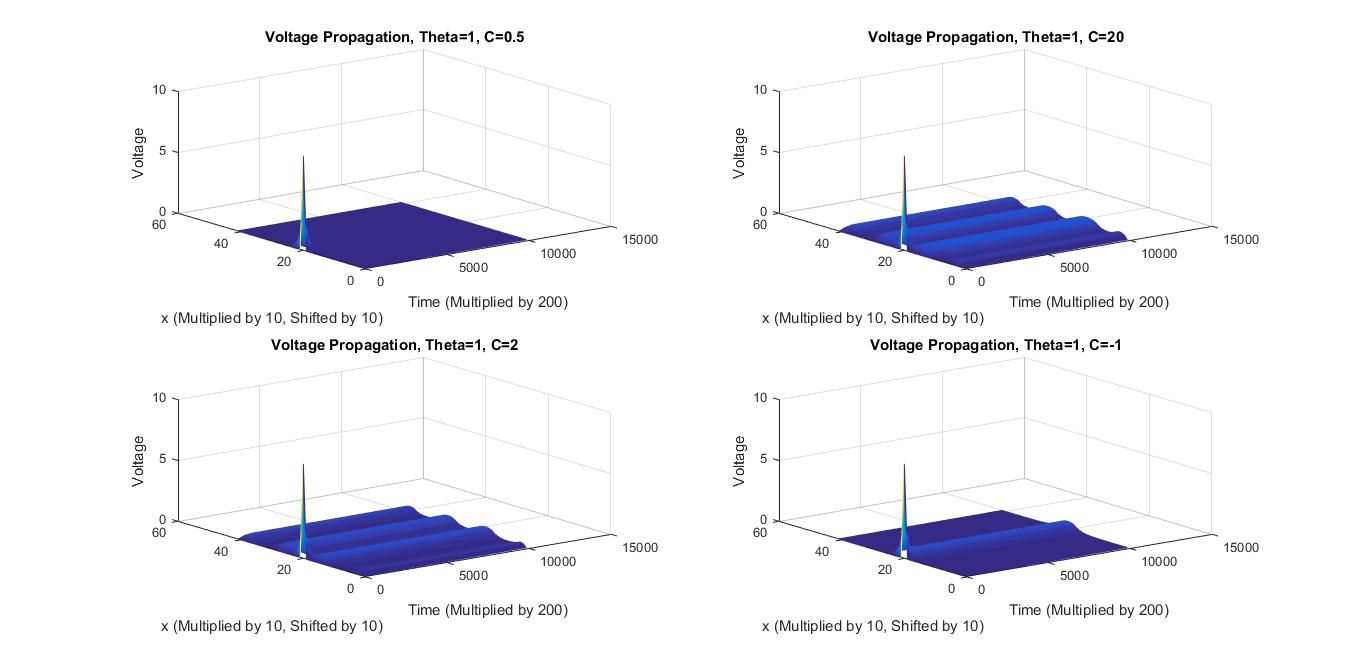
\includegraphics[width=\linewidth]{thetaone3.jpg}
  \caption{Plots of Periodically Varying Threshold, $\theta=1$}
  \label{fig:sketch7}
\end{figure}
\begin{figure}[H]
  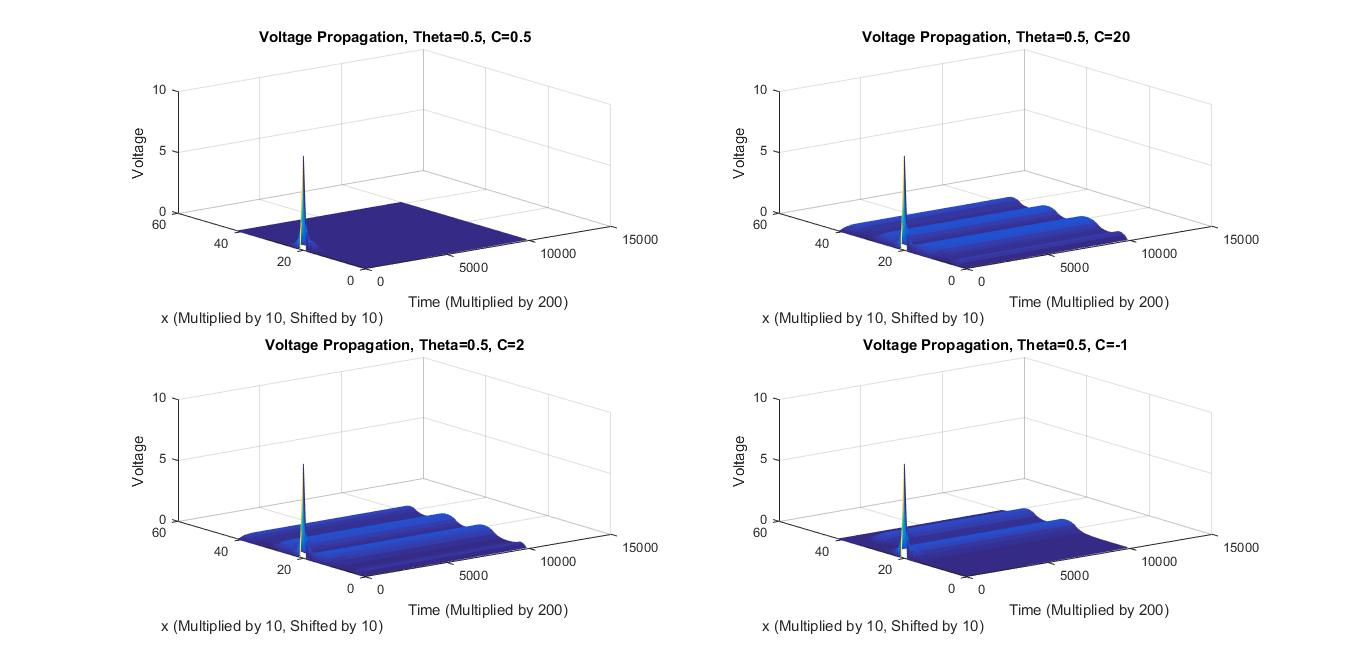
\includegraphics[width=\linewidth]{thetatwo3.jpg}
  \caption{Plots of Periodically Varying Threshold, $\theta=0.5$}
  \label{fig:sketch8}
\end{figure}
\begin{figure}[H]
  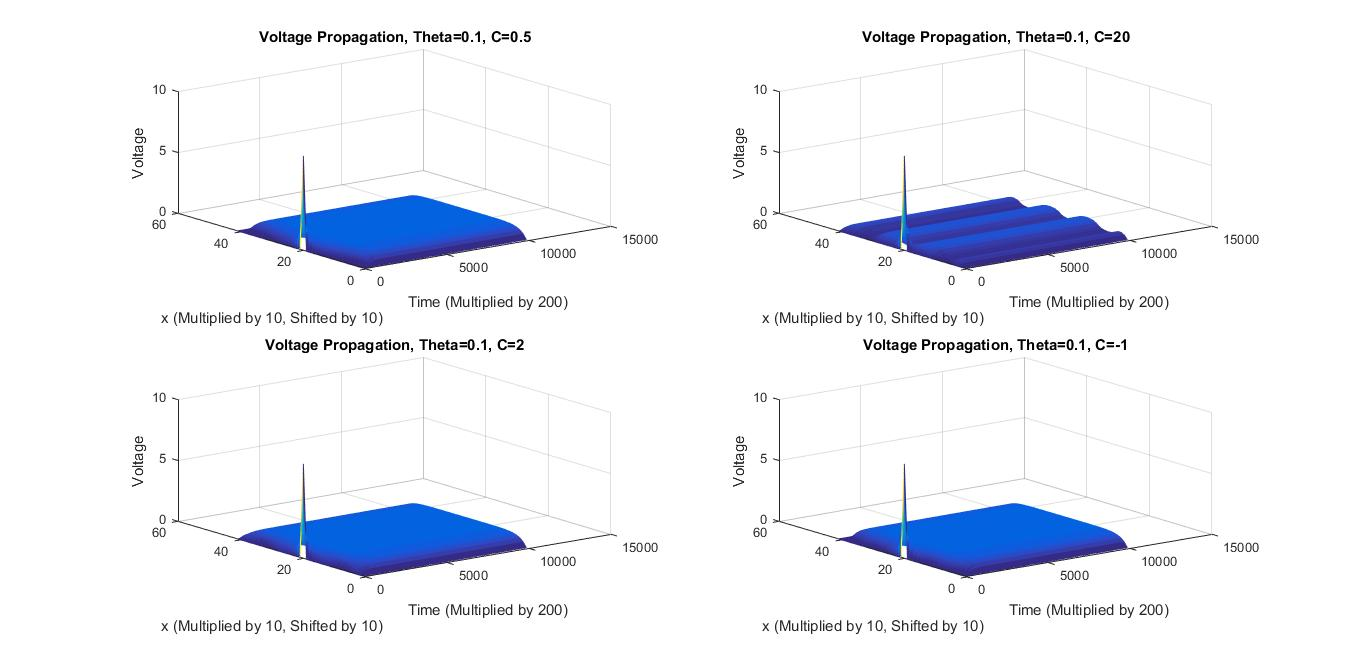
\includegraphics[width=\linewidth]{thetathree3.jpg}
  \caption{Plots of Periodically Varying Threshold, $\theta=0.1$}
  \label{fig:sketch9}
\end{figure}
It seems that if the constant $C$ is too small, not much changes from the prior solution, with $f(v(x,t))=H(v^j_i-\theta)$. This is because the constant $C$ determines how much the total value of $\theta(1+C\cos(x))$ can vary. If it has larger maginitude, it will be less likely that the variable in the Heaviside function (in this case $v_i^j$) will be larger than it when $\cos(x)=1$ or close to it, and when $\cos(x)=0$ or near this area, it is more likely that $v_i^j$ will be larger, so the value of the Heavisde function will be one. However, if $C$ is small, then these periodic fluctuations due to the cosine term will be relatively insignificant. Next, I will examine if drastically increasing the value of $C$ will have a significant effect on the same $\theta$.
\begin{figure}[H]
  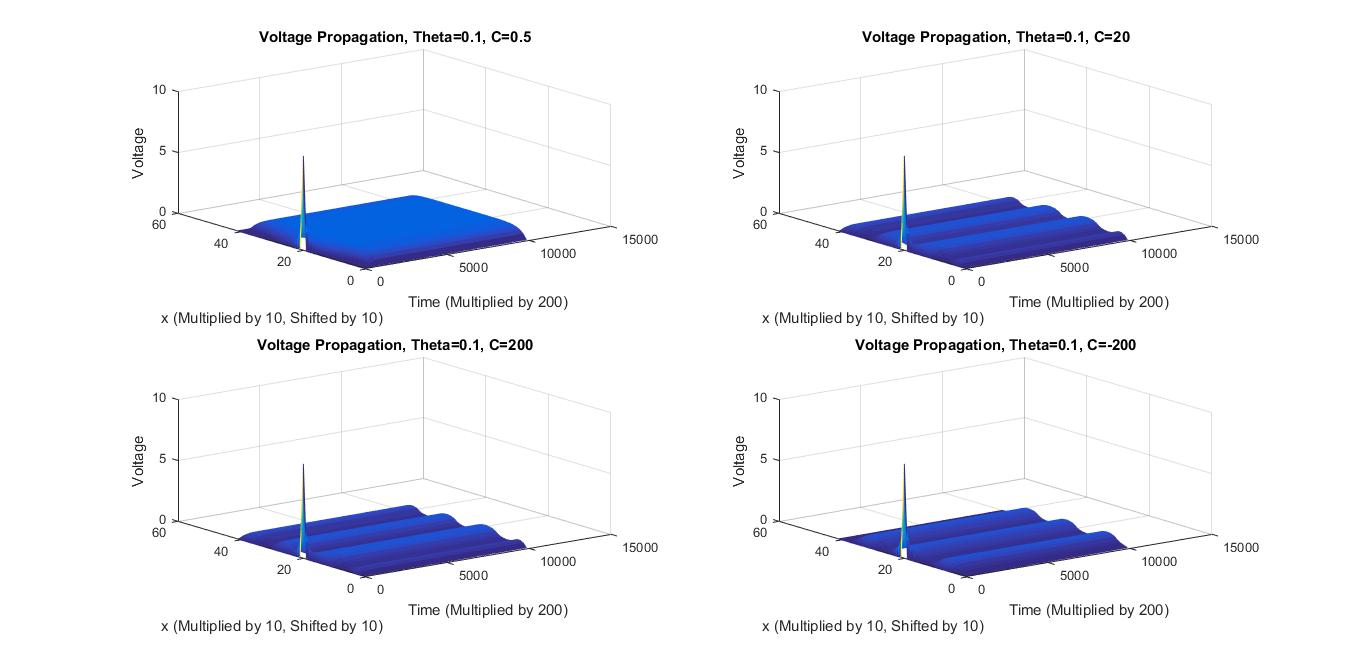
\includegraphics[width=\linewidth]{plotsomething.jpg}
  \caption{Varying $C$, $\theta=0.1$}
  \label{fig:sketch10}
\end{figure}
It appears that once $C$ is above a certain threshold, the magnitude of $C$ will not have a large effect on the waves. This makes sense because most voltage values in the orginal equation are close to zero, so they will only be larger than $\theta(1+C\cos(x))$ when $\cos(x)$ is close to zero anyway, which will result in roughly the same points being affected by the Heaviside function, no matter the magnitude of $C$. Therefore, the average speed of the front is not affected if the constant is increased drastically. \par
Also, in order to investigate if the front ever stops completely, we investigated the numerical solution on even larger intervals of x. However, when doing this, we found that waves could be seen throughoutthe entire interval of x; therefore, the front will never stop completely. 

\section{Conclusions}
In this report, we have analyzed variations of the cable equation in order to better understand the ways in which voltage can propagate throughout a neuron. After summarizing the derivation of the model, we analyzed an action potential imposed on a neuron that is experiencing ions leaking out of the cell. This was our passive membrane solution, and our models confirmed what one might expect--a large spike of voltage initially that is quickly dispersed throughout the neuron and diminished through leaking ions until the voltage goes back to zero, or its original voltage state. \par
In addition, we also analyzed a situation where the neuron has a bistable membrane which allowed us to analyze traveling waves in a solution. Our results verified our expectations, demonstrating how voltage in a neuron can propagate similar to waves approaching shore, rather than just spreading out. We were also able to numerically approximate these solutions in order to verify our results, and numerically approximate systems with more complex functions representing the opening and closing of ion channels that might be more difficult to solve analytically. Through our findings, we were able to expand our knowledge of partial differential equations and Fourier transforms by examining the cable equation and modeling voltage in a neuron. 


\pagebreak

\begin{thebibliography}{9}

\bibitem{textbook}
Haberman, Richard.
\textit{Applied Partial Differential Equations with Fourier Series and Boundary Value Problems}.
Pearson.

\bibitem{greens}
Tara LaForce.
\textit{Green's Function Course Notes}. \\
\texttt{https://web.stanford.edu/class/energy281/GreensFunctions.pdf}

\bibitem{perturb}
University of California, Davis.
\textit{Linearizing Equations About Rest Points}. \\
\texttt{https://www.math.ucdavis.edu/~temple/MAT22C/LecturesMat22CW15/5-\\LinearizedEquationsAboutRestPoints-22C-W15.pdf}

\bibitem{fourier}
USPAS.
\textit{Table of Fourier Transform Pairs}. \\\texttt{http://uspas.fnal.gov/materials/11ODU/FourierTransformPairs.pdf}

\end{thebibliography}
















\end{document}